%\mode<all>
%
%Los cálculos ab initio consisten, a grandes rasgos, en resolver la ecuación de
%Schrödinger para el sistema de electrones e iones particular. Sin embargo, aún para
%sistemas realmente pequeños la cantidad de grados de libertad hace que el sistema se
%vuelva inmanejable.

\mode*
\begin{frame}<presentation>[label=FrameMotivacion]
  \frametitle{Escala Atomística}

  \centering

  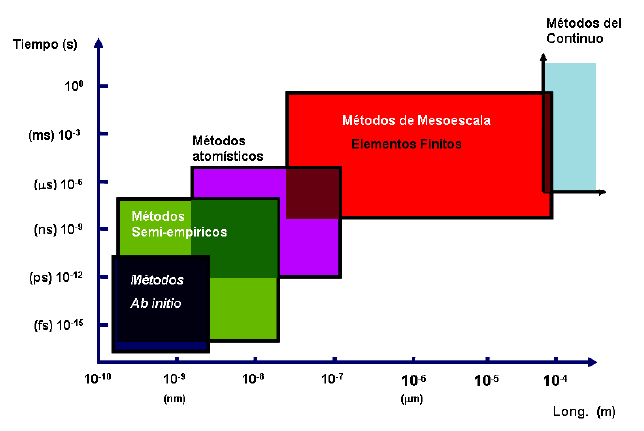
\includegraphics[width=0.8\textwidth]{Figures/Escalas.png}

\end{frame}

%\mode<article>

%Existen estrategias para simplificar el problema. La DFT (Sholl & Steckel 2009; Koch
%& Holthausen 2001) se basa en dos teoremas que Hohenberg y Kohn (HK) enunciaron
%en la decada de 1960 (Hohenberg & Kohn 1964). Estos autores se basan en la idea de
%que en principio toda la información física de la función de onda de un sistema de
%muchos electrones esta contenida en la densidad electrónica. Si $\psi$
% es la función de onda que resuelve la ecuación de Schrödinger del sistema de $N$
% electrones, entonces la densidad electrónica puede definirse como


\mode*
\begin{frame}<presentation>[label=FrameTeorema1]
 \frametitle{Aproximaciones y Teoremas de Hohenverg y Kohn}

 \begin{itemize}

   \item Los núcleos atómicos son suficientemente pesados como para poder considerarlos un potencial externo fijo respecto del sistema electrónico.
     (Born-Oppenheimer)

   \item Toda la información física se encuentra en la densidad electrónica.

   \item La energía del sistema es una funcional de la densidad electrónica.

     $$ E = E[\rho] $$

   \item La densidad electrónica real del sistema minimiza su energía, dado el potencial externo.

     $$ E[\rho_0 + \delta \rho ] \ge E[\rho_0]$$

 \end{itemize}

\end{frame}

\mode<all>
